\chapter{Системийн шаардлага}

Уг бүлэг нь системийн хэрэглэгчийн зүгээс тавигдах шаардлагыг тодорхойлж, тухайн гаргасан шаардлагууд дээрээ үндэслэн UX судалгаа хийсэн талаарх гарах ба хэрэглэгч суурьтай интерфейс дизайн гаргахад тулгарсан асуудлуудыг товч дурдлаа.

\section{Шаардлагын шинжилгээ}

\subsection{Хэрэглэгчид}

Интернер сүлжээ ашиглан мэдээлэл авдаг, бусадтай хуваалцдаг бүх төрлийн хэрэглэгчид

\subsection{Функционал шаардлагууд}

\begin{itemize}
	\item Веб нь бусад веб холбоосуудыг дангаар нь болон бүлэглэж оруулах боломжтой байх
	\item Нийт хэрэглэгчдийн оруулсан веб холбоосууд, хэрэглэгчдийн мэдээллээс түлхүүр үгээр хайлт хийх боломжтой байх
	\item Хэрэглэгч бүлэглэж оруулсан холбоосуудаа бусад хүмүүстэй хуваалцах боломжтой байх
	\item Хэрэглэгч платформ дээрх дурын хүнээ дагах, түүний оруулсан веб холбоосуудыг харах боломжтой байх
	\item Бусад хүмүүсийн оруулсан веб холбоосууд дээр хэрэглэгч үнэлгээ өгдөг боломжтой байх
\end{itemize}

\subsection{Функционал бус шаардлагууд}

\begin{itemize}
	\item Веб нь хэрэглэгч ашиглахад хялбар интерфейстэй байх
	\item Интерфейс дизайн нь түлхүү цагаан болон брэнд өнгийг хадгалсан шинэлэг дизайнтай байх
	\item Веб дээр нийтлэл оруулах үед бусад веб холбоосуудын Open Graph мэдээллийг 500 миллсекундэд багтаан авдаг байх
	\item Веб нь бүхий л төрлийн төхөөрөмжүүд дээр интерфейсийн алдаагүй ажиллах Responsive бүтэцтэй байх
	\item Веб холбоос оруулах үед дээд тал нь хоёр hashtag ашигладаг байх
	\item Хэрэглэгч хэдэн ч удаа веб холбоос оруулах боломжтой байх
\end{itemize}

\section{UX судалгаа}

Хэрэглэгч суурьтай дизайн гаргахад хамгийн чухал зүйл бол хэрэглэгчээ танин тэдгээрээс судалгаа авах, гаргасан үр дүнгээ ашиглан дизайнаа хөгжүүлэх, тодорхой тооны хэрэглэгчээр туршиулж сайжруулах үе шат юм. Миний хувьд эхлээд хэрэглэгчээ тодорхойлж, тус бүрийн Use Case-г гарган түүн дээ зориулан Wireframe хувилбар гаргасан. 

\subsection{User Personas}

\subsubsection{Persona 1 - Болорчулуун}

\begin{figure}[h]
	\centering
	
\includegraphics[width=15cm]{images/persona1-bolorchuluun.png}
	\caption{Persona 1 - Болорчулууны мэдээлэл}
	\label{fig:persona1}
\end{figure}

\textbf{Use Case}

\begin{itemize}
	\item Өглөө ажил дээрээ эхний 20 минут мэргэжилтэйгээ холбоотой нийтлэлүүд унших дуртай
	\item Веб хөтөч дээрээ таалагдсан эсвэл дараа нь унших ёстой холбоосуудаа bookmark хийж хадгалж авдаг боловч зөвхөн ажлын компьютер дээр л тэдгээр холбоос маань хадгалагддаг. Өөр рүүгээ веб холбоосоо цуглуулж явуулахаас залхуу хүрдэг
\end{itemize}

\subsubsection{Persona 2 - Шүрэнцэцэгийн мэдээлэл}

\begin{figure}[h]
	\centering
	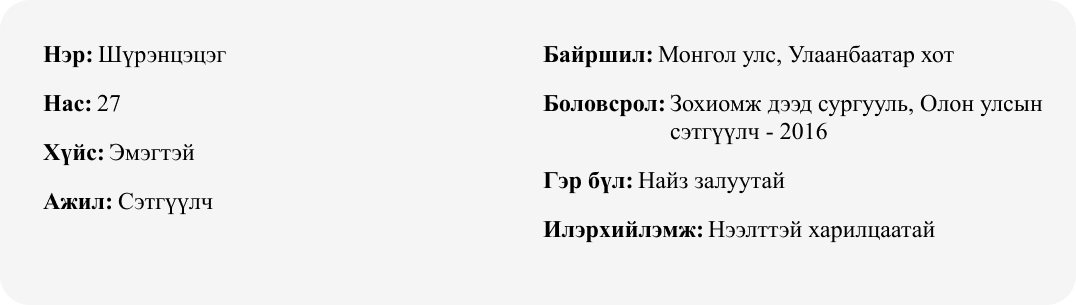
\includegraphics[width=15cm]{images/persona2-shurentsetseg.png}
	\caption{Persona 2 - Шүрэнцэцэг}
	\label{fig:persona1}
\end{figure}

\textbf{Use Case}

\begin{itemize}
	\item Миний хувьд мэдээгээ бэлтгэхдээ дийлэнхдээ интернет дэх эх сурвалжуудаас бэлтгэдэг. Нэг асуудал байдаг маань эх сурвалж авдаг хэдхэн вэбсайт дунд л эргэлдэж байгаа.
	\item Олсон мэдээллүүдээ хамт ажиллаж буй хүмүүс рүүгээ явуулахдаа Telegram ашиглан нэг нэгээр нь хуулж тавин явуулдаг. Хүн болгон руу ингэж явуулах нь надад төвөгтэй байдаг
\end{itemize}

\subsection{Гаргасан интерфейс загварын эхний хувилбар}

Уг хэсэг дээр хэрэглэгчдийн Use Case, Empathy загвар дээр тулгуурлаж Wireframe болон High Fidelity түвшний интерфейс загвар гаргасан. Жишээ зургууд оруулав

\begin{figure}[h]
	\centering
	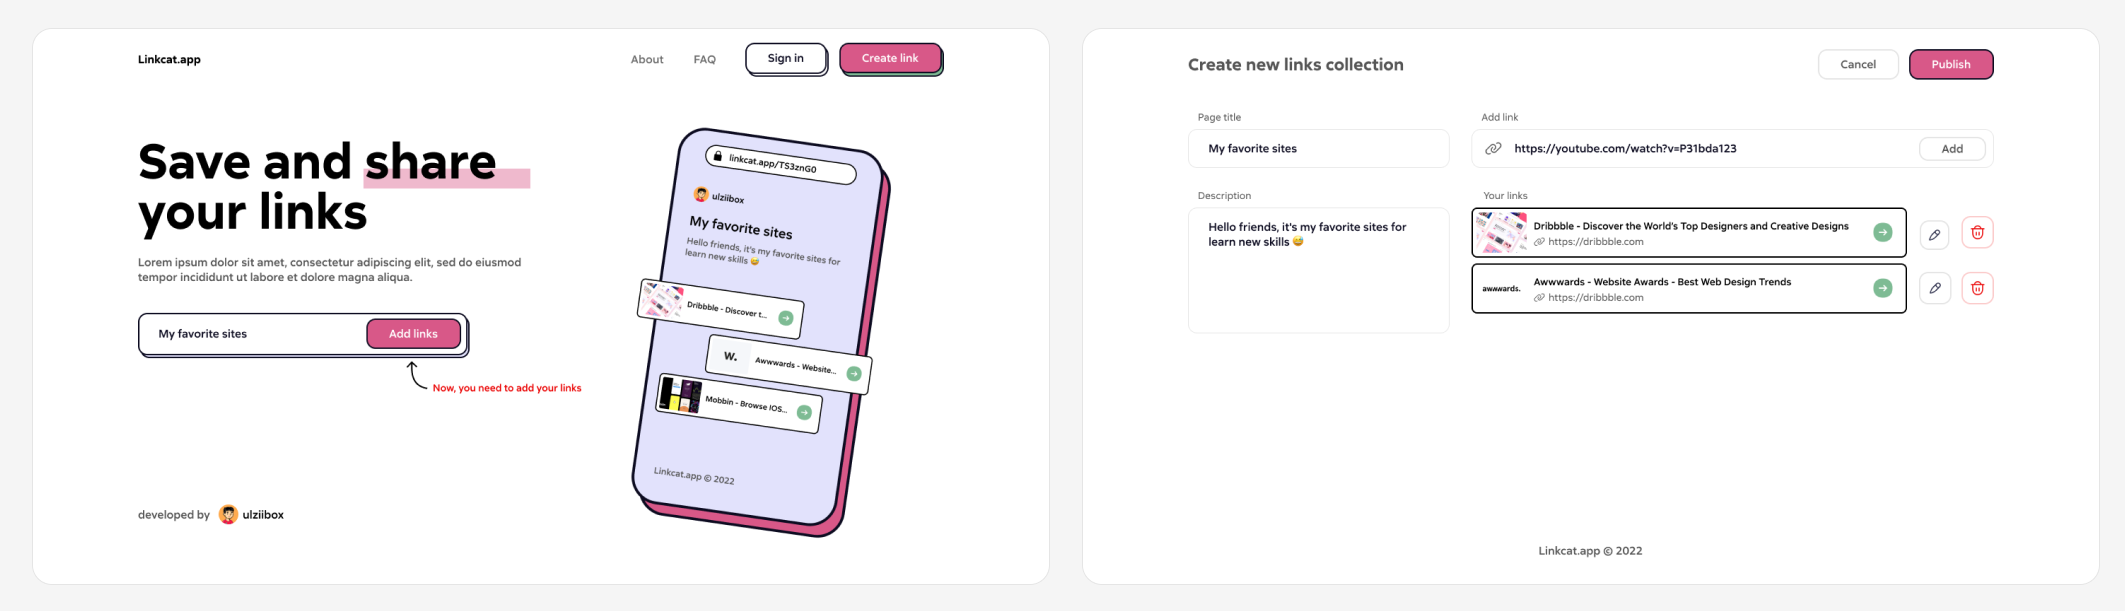
\includegraphics[width=0.5]{images/01-interface.png}
	\caption{Нүүр хуудас болон веб холбоос оруулах flow}
	\label{fig:interface1}
\end{figure}

\begin{figure}[h]
	\centering
	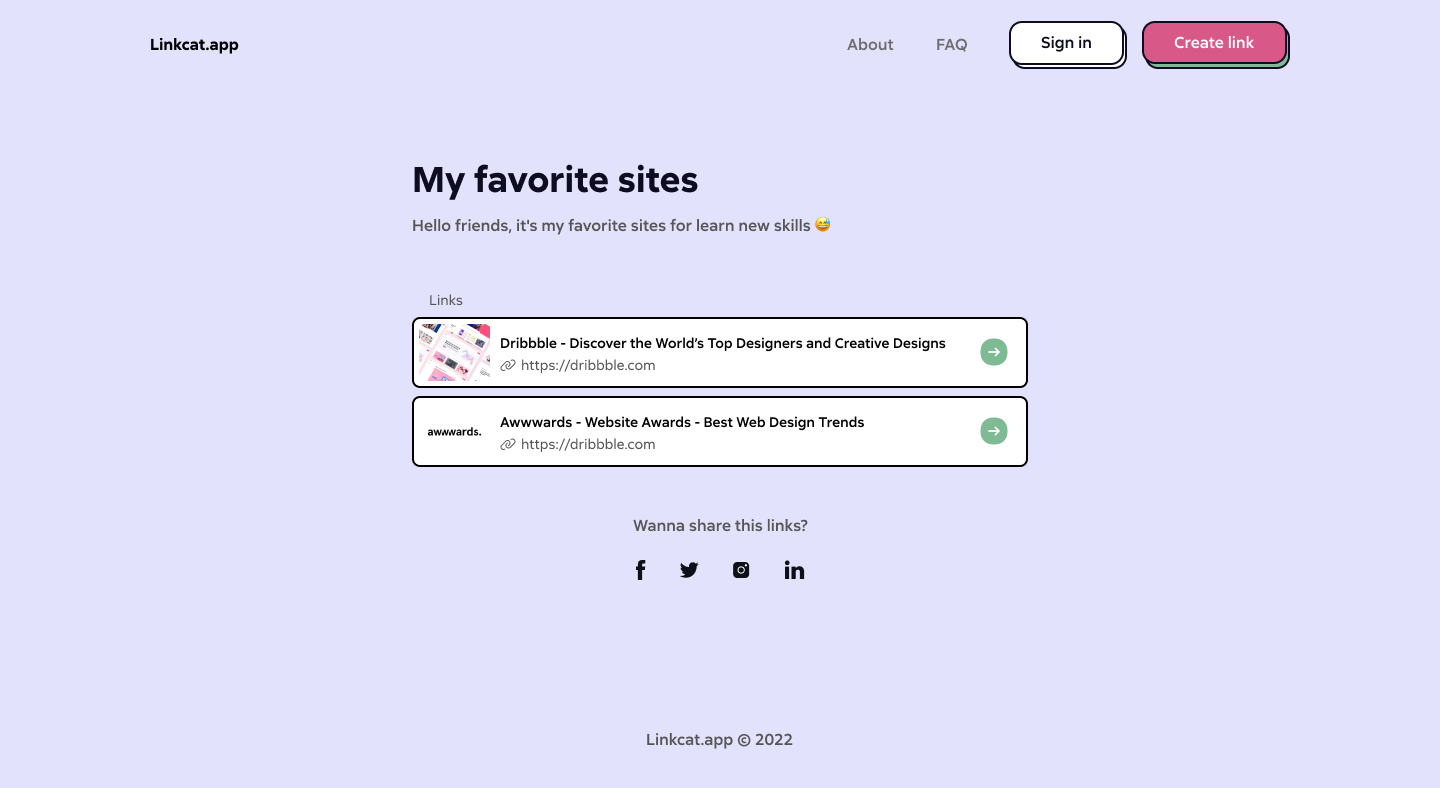
\includegraphics[width=15cm]{images/03-interface-page.png}
	\caption{Оруулсан веб холбоосуудыг бусад хэрэглэгчид харах хуудас}
	\label{fig:interface1}
\end{figure}
